\documentclass[12pt,a4paper]{article}


% Packages
%======================================
% Page Geometry
\usepackage[DIV=14,BCOR=2mm,headinclude=true,footinclude=false]{typearea}
%======================================
% Document spacing
% Line spacing
\usepackage{setspace}
\setstretch{1.2}
% Paragraph spacing
\usepackage[skip=2.5pt, indent=12pt]{parskip}
%======================================
% Headers and footnotes
\usepackage{fancyhdr}
%======================================
% Math packages
\usepackage{tikz}
\usepackage{physics}
\usepackage{tikz-cd}
\usepackage{mathtools}
\usepackage{amsmath,amssymb}
% Quotient space
\newcommand{\bigslant}[2]{{\raisebox{.2em}{$#1$}\left/\raisebox{-.2em}{$#2$}\right.}}
%======================================
% Theorem environments
\usepackage{amsthm}
\newtheorem{theorem}{Theorem}[section]
\newtheorem{lemma}[theorem]{Lemma}
\newtheorem{corollary}{Corollary}[theorem]
% Definition style
\theoremstyle{definition}
\newtheorem{definition}{Definition}[section]
% Remark style
\theoremstyle{remark}
\newtheorem{remark}{\textit{Remark}}[section]
% Example style
\theoremstyle{definition}
\newtheorem{example}{Example}[section]
%======================================
% German ß ä ö ü
\usepackage[T1]{fontenc}
\usepackage[main=english,german]{babel}
%======================================
% Color
\usepackage{xcolor}
\definecolor{TUColor}{cmyk}{0, 1.0, 0.99, 0.40} % TU Dark Red
\definecolor{CitationColor}{cmyk}{0.9, 0.6, 0.0, 0.6} % Dark Blue
\definecolor{RichBlack}{cmyk}{0.75, 0.68, 0.67, 0.9}
%======================================
% Hyper links and references
\usepackage{hyperref}
\hypersetup{
    colorlinks,
    urlcolor={CitationColor},
    citecolor={CitationColor},
    linkcolor={RichBlack}
}
%======================================
% Citations
\usepackage[nobreak]{cite}
%======================================
% Images
\usepackage{float}
\usepackage{graphicx}
\graphicspath{{./images/}}
% Captions
\usepackage{subcaption}
\renewcommand\thesubfigure{\roman{subfigure}}
%======================================
% For Title page
\usepackage{tabularx,booktabs}
%======================================
% Fancy boxes
\usepackage[most]{tcolorbox}
\tcbuselibrary{skins,breakable}
\newtcolorbox{mybox}[2][]{breakable, sharp corners, boxrule=0mm, leftrule=2mm, boxsep=0mm, arc=0mm, outer arc=0mm, opacityframe=0}
%======================================


\begin{document}
%===========================================================
% General settings
% Font color
\color{RichBlack}
% Redefine header "fancy" style
\fancypagestyle{fancy}{
    \fancyhead{}
    \fancyfoot{}
    \fancyhead[LE,RO]{\footnotesize\itshape\nouppercase{\rightmark}}
    \fancyhead[LO,RE]{\footnotesize\itshape\nouppercase{\leftmark}}
    \fancyfoot[C]{\footnotesize\itshape\nouppercase\thepage}
    \renewcommand{\headrulewidth}{0.4pt}
    \renewcommand{\footrulewidth}{0.0pt}
}
\fancypagestyle{tocstyle}{
  \fancyhead{}
  \fancyfoot{}
  \renewcommand{\headrulewidth}{0.4pt}
  \renewcommand{\footrulewidth}{0.0pt}
}
%===========================================================


% Title page
%===========================================================
\begin{titlepage}
% Defines a new command for horizontal lines, change thickness here
\newcommand{\HRule}{\rule{\linewidth}{0.5mm}}
\begin{center}


\includegraphics[width=0.15\textwidth]{TU-Berlin-Logo.png}\\[1cm]
\begin{otherlanguage}{german}
\textsc{\LARGE Technische Universit"at Berlin}\\[1.5cm]
\textsc{\large Fakult\"at 2}\\[0.5cm]
\textsc{\large Institut f\"ur Mathematik}\\[0.5cm]
\end{otherlanguage}

% Title
\setlength{\aboverulesep}{10pt}
\setlength{\belowrulesep}{13pt}
\begin{tabularx}{\textwidth}{ >{\centering\arraybackslash}X}
\midrule[0.5mm]
\huge\bfseries Circular cross sections of quadrics\\
\midrule[0.5mm]
\end{tabularx}

% Author and supervisor
\begin{minipage}{0.4\textwidth}
    \begin{flushleft}
        \large
        \textit{\textcolor{TUColor}{Author}}\\
        Sara \textsc{Samy}
    \end{flushleft}
\end{minipage}
~
\begin{minipage}{0.4\textwidth}
    \begin{flushright}
        \large
        \textit{\textcolor{TUColor}{Supervisor}}\\
        Dr. Jan \textsc{Techer}
    \end{flushright}
\end{minipage}

% Position the date 3/4 down the remaining page
\vspace{260 pt}
{\large\today}
\end{center}
\end{titlepage}
%===========================================================


%===========================================================
% Set Abstract page style to "fancy"
\pagestyle{fancy}
\section*{Abstract}
\label{sec:abstract}

\pagebreak
%===========================================================
% Set TOC page style to "tocstyle"
\pagestyle{tocstyle}
\renewcommand{\contentsname}{Contents}
\tableofcontents
\pagebreak
%===========================================================
\listoffigures
\pagebreak
%===========================================================
% Set all following pages style to "fancy"
\pagestyle{fancy}
\section{Introduction}
\label{sec:introduction}
\pagebreak
%===========================================================
\section{Circular sections of quadrics}
\label{sec:circular-sections-of-quadrics}

In this paper, the term \textit{quadric} stands for ellipsoids (including spheres), hyperboloids, and paraboloids. We do not consider singular surfaces of degree two like quadratic cones and cylinders or degenerate cases like planes or pairs of planes (Appendix \ref{appendix:quadrics}).

\subsection{Complex projective space}
\label{subsec:complex-projective-space}

Before we start investigating circles on quadrics, we briefly recall a few facts about the $n$-dimensional (complex) projective space. A point in the complex projective space $\mathbb{C}\mathbb{P}^{n}$ is determined by $n + 1$ elements $(z_{0}, \dots, z_{n})$ of the field $\mathbb{C}$, not all simultaneously zero. \\
Two $(n + 1)$-tuples $(z_{0}, \dots, z_{n})$ and $(z'_{0}, \dots, z'_{n})$  determine the same point if and only if there exists $\lambda \in \mathbb{C} \setminus \{ 0 \}$ such that $z_{i} = \lambda z_{i}'$ for $i = 0, \dots, n$. This defines an equivalence relation on $\mathbb{C}^{n + 1} \setminus \{ 0 \}$, and we can identify the complex projective space $\mathbb{C}\mathbb{P}^n$ with the quotient space of $\mathbb{C}^{n + 1} \setminus \{ 0 \}$ under this equivalence relation:
\[
    \mathbb{C}\mathbb{P}^n \cong \bigslant{\left( \mathbb{C}^{n + 1} \setminus \{ 0 \} \right)}{\sim}.
\]
Any $(n+1)$-tuple defining a point $P$ is called a set of \textit{homogeneous coordinates} of $P$, and we write $P = [z_{0},\dots, z_{n}]$.\par

There is a natural embedding $\mathbb{C}^n \hookrightarrow \mathbb{C}\mathbb{P}^n$ which sends an affine point $(z_{0}, \dots, z_{n-1}) \in \mathbb{C}^n$ to its equivalent class $[z_{0},\dots, z_{n-1}, 1] \in \mathbb{C}\mathbb{P}^n$.  We get in this way all points with $z_{n} \neq 0$ since a point $[z_{0}, \dots, z_{n}]$ with $z_{n} \neq 0$ corresponds to the affine point $(z_{0}/z_{n}, \dots, z_{n-1}/z_{n}) \in \mathbb{C}^{n}$. The points of the complementary set with $z_{n} = 0$ are called \textit{points at infinity}. This notion depends on the choice of the coordinate $z_{n}$. In fact, $\mathbb{C}\mathbb{P}^n$ contains $n + 1$ isomorphic copies of the affine space $\mathbb{C}^n$:
\[
U_{i} = \left\{ \left[ \frac{z_{0}}{z_{i}}, \dots, \frac{z_{n}}{z_{i}} \right] : z_{j} \in \mathbb{C} \ \text{for} \ j=0, \dots, n \ \text{and} \ z_{i} \neq 0 \right\} \cong \mathbb{C}^n, \quad \quad i=0, \dots, n.
\]
Every point $P \in \mathbb{C}\mathbb{P}^n$ is contained in at least one of these pieces, and can be written down in the affine coordinates of that piece [Figure~\ref{fig:affine-patches-diagram}].\par

\begin{figure}[H]
    \centering
    
\includegraphics[width=0.6\textwidth]{affine-patches.png}
    \caption{$\mathbb{C}\mathbb{P}^2$ realised as the gluing of three affine patches $U_0, U_1$, and $U_2$ \cite{toricfanovarieties2005}.}
    \label{fig:affine-patches-diagram}
\end{figure}

The planes of the generating circles are parallel \cite[\textcolor{CitationColor}{\textit{Lemma~2.1}}]{nilovSurfaceContainingLine2011}, and intersect the surface only at the points of the circles \cite[\textcolor{CitationColor}{\textit{Lemma~2.6}}]{nilovSurfaceContainingLine2011}.

\pagebreak
%===========================================================
\section{Families of confocal quadrics}
\label{sec:confocal-quadrics}

\begin{definition}[Confocal quadrics]
\label{def:confocal-quadrics}
Two quadrics are \textit{confocal}, sometimes also referred to as \textit{homofocal}, if they have common axes and intersect each plane of symmetry along confocal conics.
\end{definition}
A classical system of confocal quadrics in Euclidean space $\mathbb{R}^3$ is composed of three families of quadrics given by

\pagebreak
%===========================================================
\section{Lines of curvature on confocal quadrics}
\pagebreak
%===========================================================
\section{Diagonally related nets on surfaces}
\label{sec:diagonally-related-nets}

We start by defining nets on surfaces. Mutually diagonal nets on surfaces were introduced in \cite{MutuallyDiagonalNets2019}.

\begin{definition}[Nets on surfaces]
\label{def:nets-on-surfaces}
A net $\mathcal{N}$ on a surface $\Sigma$ is a pair of one-parameter families of curves on $\Sigma$, such that for every point on $\Sigma$ there exists exactly one curve from each of the two families through that point.
\end{definition}

\begin{remark}[]
\label{rm:label}
Let $\mathcal{N} = \left( (\alpha_{s_{1}})_{s_{1} \in I_1}, (\beta_{s_{2}})_{s_{2} \in I_2} \right)$ be a net on a surface
$\Sigma$, and $P$ a point on the surface then there exists a unique pair $(s_{1}, s_{2}) \in I_{1}\times I_{2}$ such that
\[
    P = \alpha_{s_1} \cap \beta_{s_2}
\]
We call $(s_1, s_2)$ the \textit{coordinates of the point $P$ with respect to the net $\mathcal{N}$}. Note that these coordinates alone do not uniquely determine the points on the surface, especially that we don't assume that each two curves from different families of $\mathcal{N}$ intersect in one unique point. However, the net together with a specific parameterization of its curves uniquely determine the points of the surface.
\end{remark}

\begin{example}
\label{ex:coordinate-lines-form-net-on-surfaces}
Let $\varphi : I_{1} \times I_{2} \subset \mathbb{R}^2 \to \mathbb{R}^3$ be a parameterization of a surface. Then its
coordinate lines, i.e. the curves
\begin{align*}
    \varphi_{u_0} : I_{2} \to \mathbb{R}^3 &\quad \quad \varphi_{u_0}(v) = \varphi(u_0, v), \text{ and} \\
    \varphi_{v_0} : I_{1} \to \mathbb{R}^3 &\quad \quad \varphi_{v_0}(u) = \varphi(u, v_0)
\end{align*}
defined for each fixed $u_{0} \in I_1, v_{0} \in I_2$ constitute a net on the surface $\varphi\left( I_1 \times I_{2}
\right) \subset \mathbb{R}^3$.
\end{example}

\begin{example}
\label{ex:circular-sections-form-nets-on-quadrics}
In \hyperref[sec:circular-sections-of-quadrics]{Section Two} we proved that quadrics contain two circles through each point. Thus, the circular sections quadrics form a net on quadrics.
\end{example}

\begin{figure}[!tbp]
  \begin{subfigure}[b]{0.5\textwidth}
    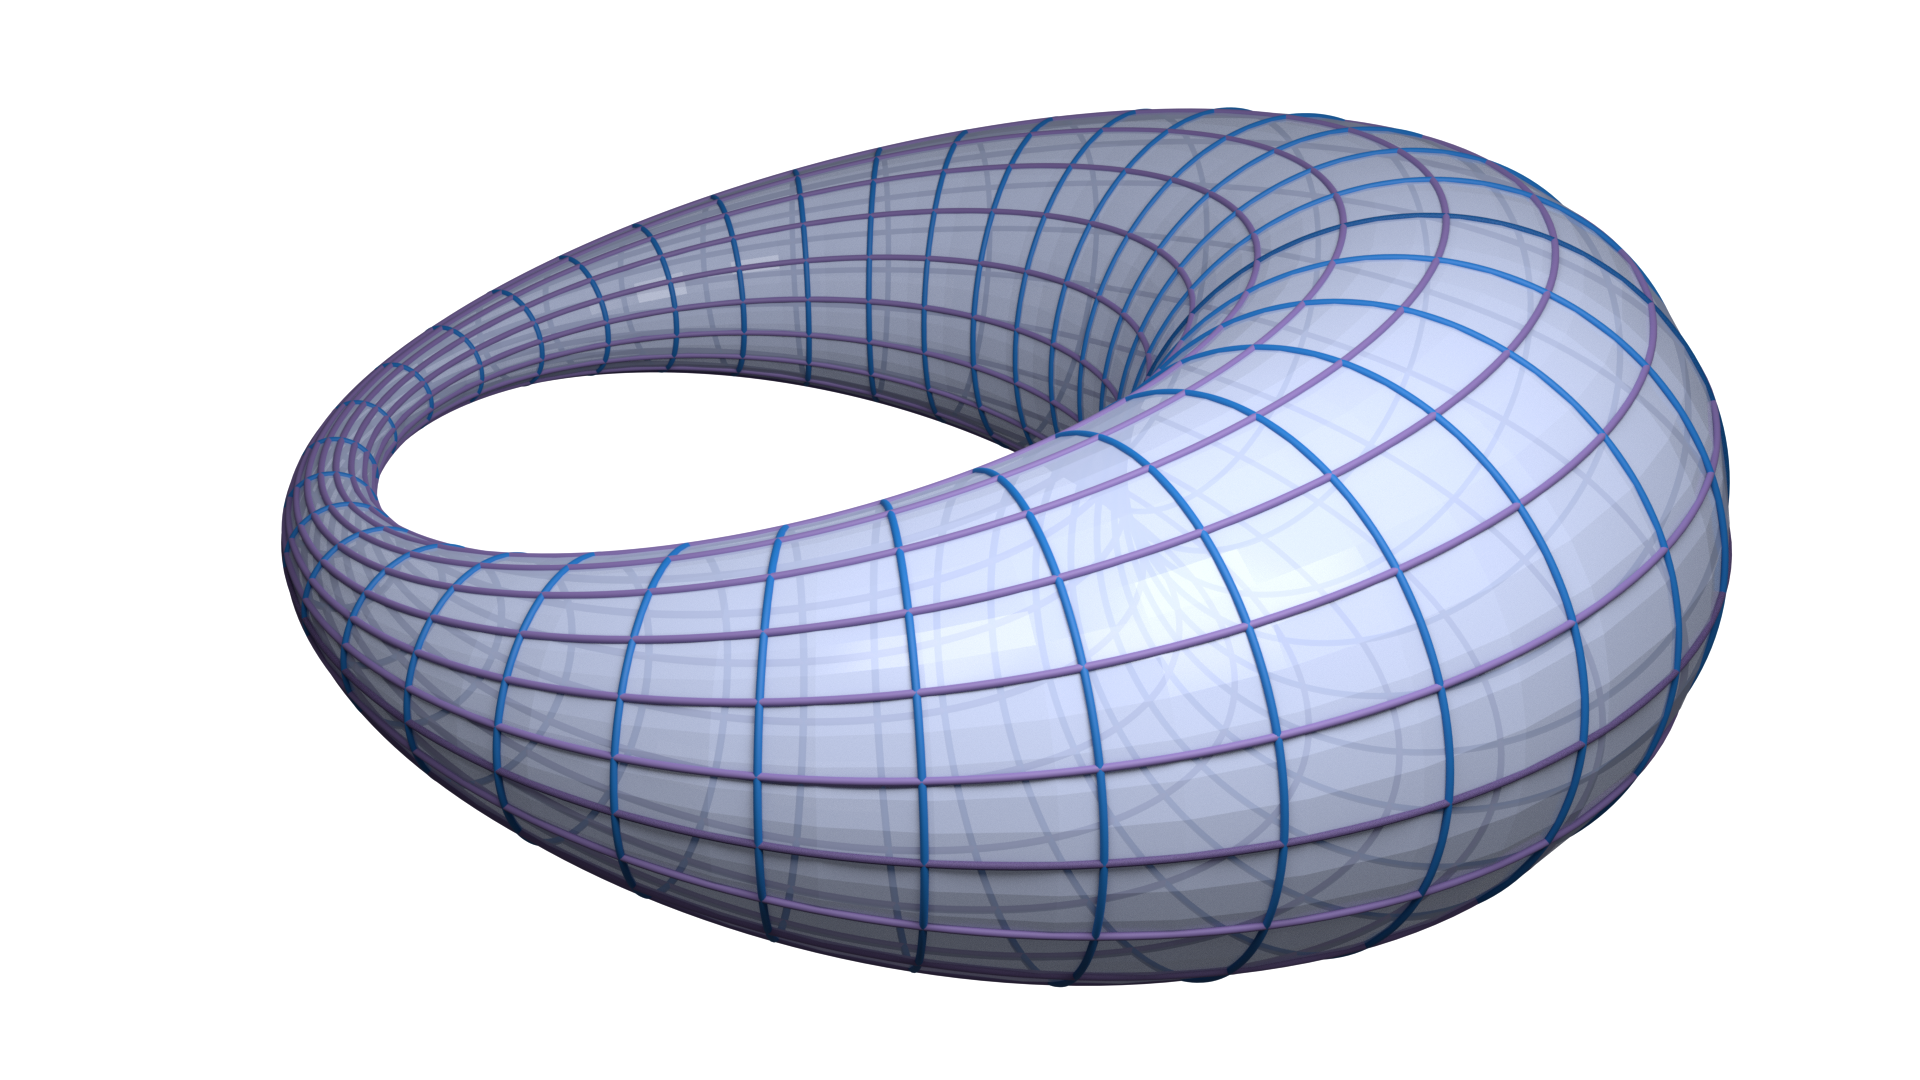
\includegraphics[width=\textwidth]{Dupin-net.png}
    \caption{ellipto-hyperbolic}
    \label{fig:ellipto-hyperbolic-cyclides}
  \end{subfigure}
  \hfill
  \begin{subfigure}[b]{0.5\textwidth}
    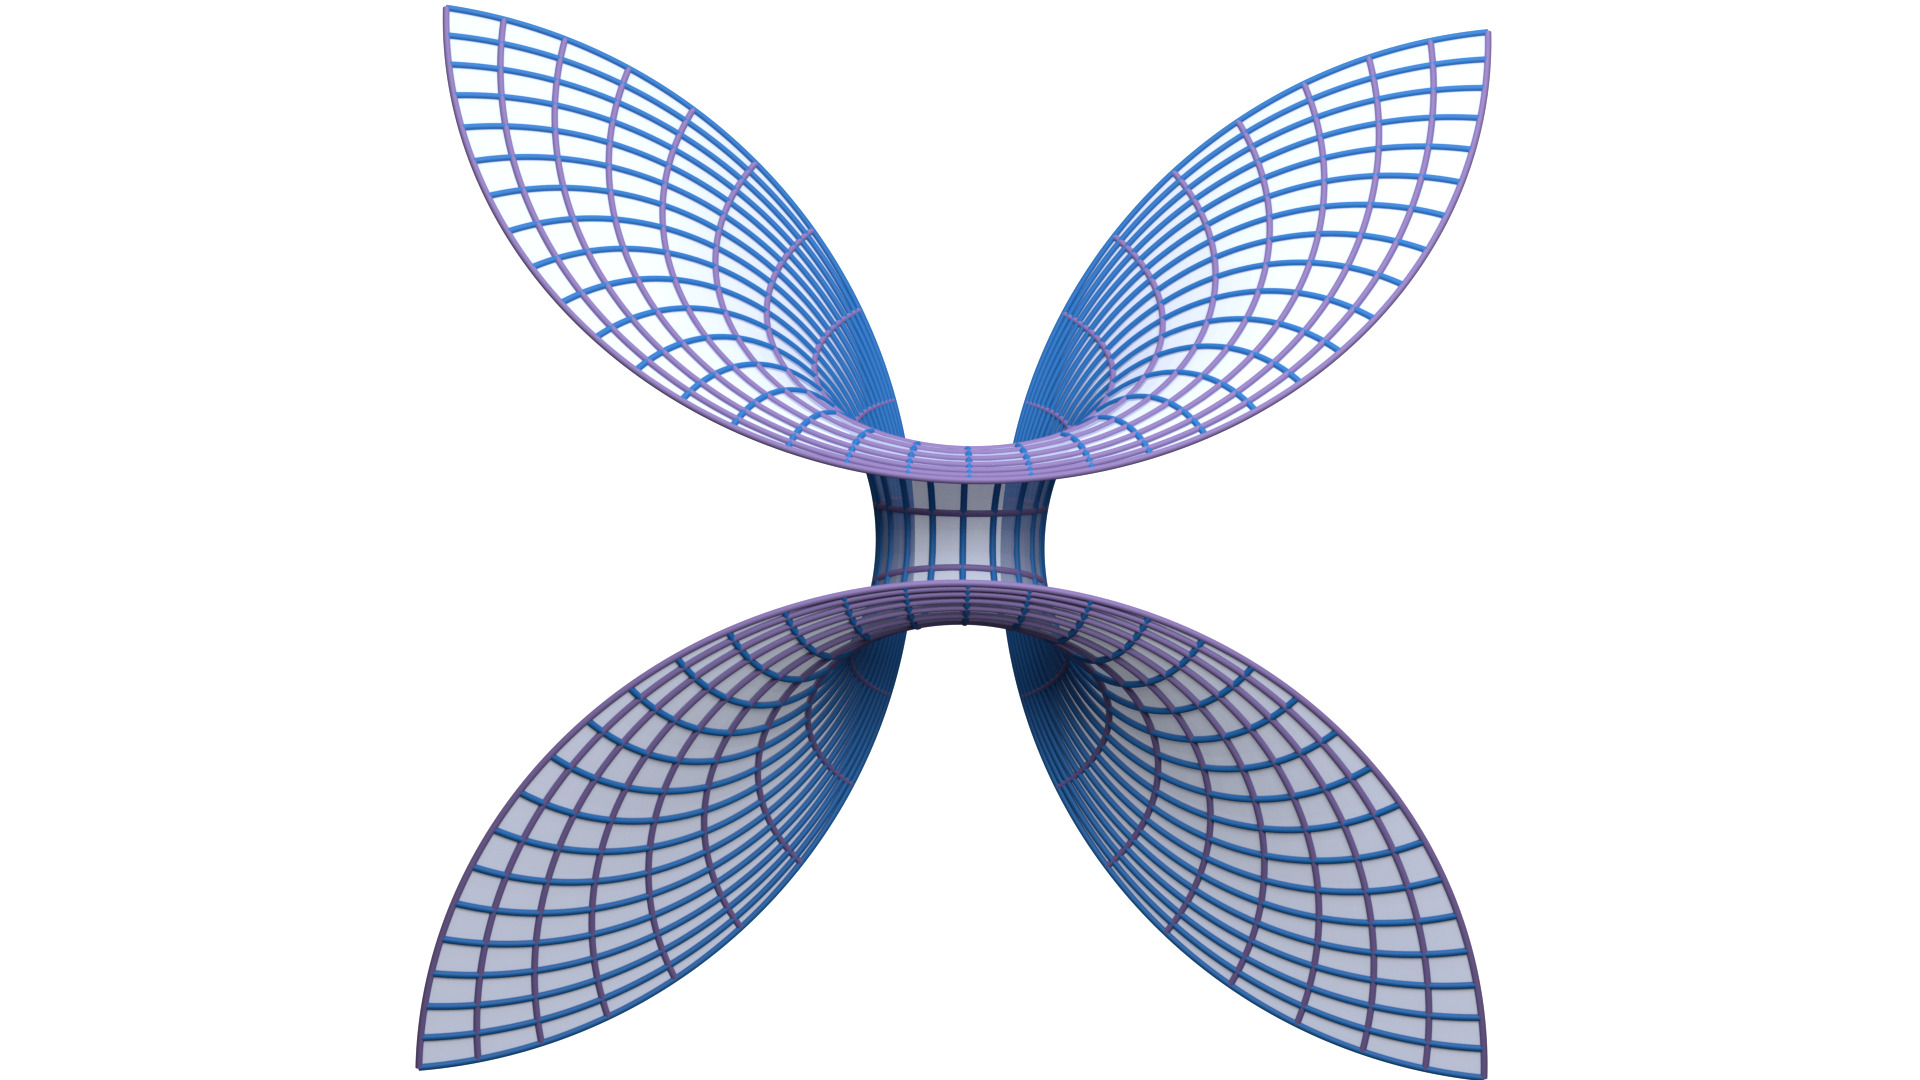
\includegraphics[width=\textwidth]{Dupin-net-2.png}
    \caption{parabolic}
    \label{fig:parabolic-cyclides}
  \end{subfigure}
  \caption{Dupin Cyclides}
\end{figure}

\begin{definition}[Diagonally related nets on surfaces]
\label{def:diag-nets-on-surfaces}
Let $\mathcal{N}_{1}$ and $\mathcal{N}_{2}$ be two nets on a surface $\Sigma$. Then $\mathcal{N}_{2}$ is called diagonal
to $\mathcal{N}_{1}$ if the following condition is satisfied whenever any four curves of $\mathcal{N}_{1}$ form a
(combinatorial) quadrilateral:\\
\begin{mybox}{}
If one pair of opposite vertices is connected by a curve from $\mathcal{N}_{2}$, then the other pair of opposite vertices is connected by a curve from $\mathcal{N}_{1}$.
\end{mybox}
\end{definition}

\begin{figure}[h]
    \centering
    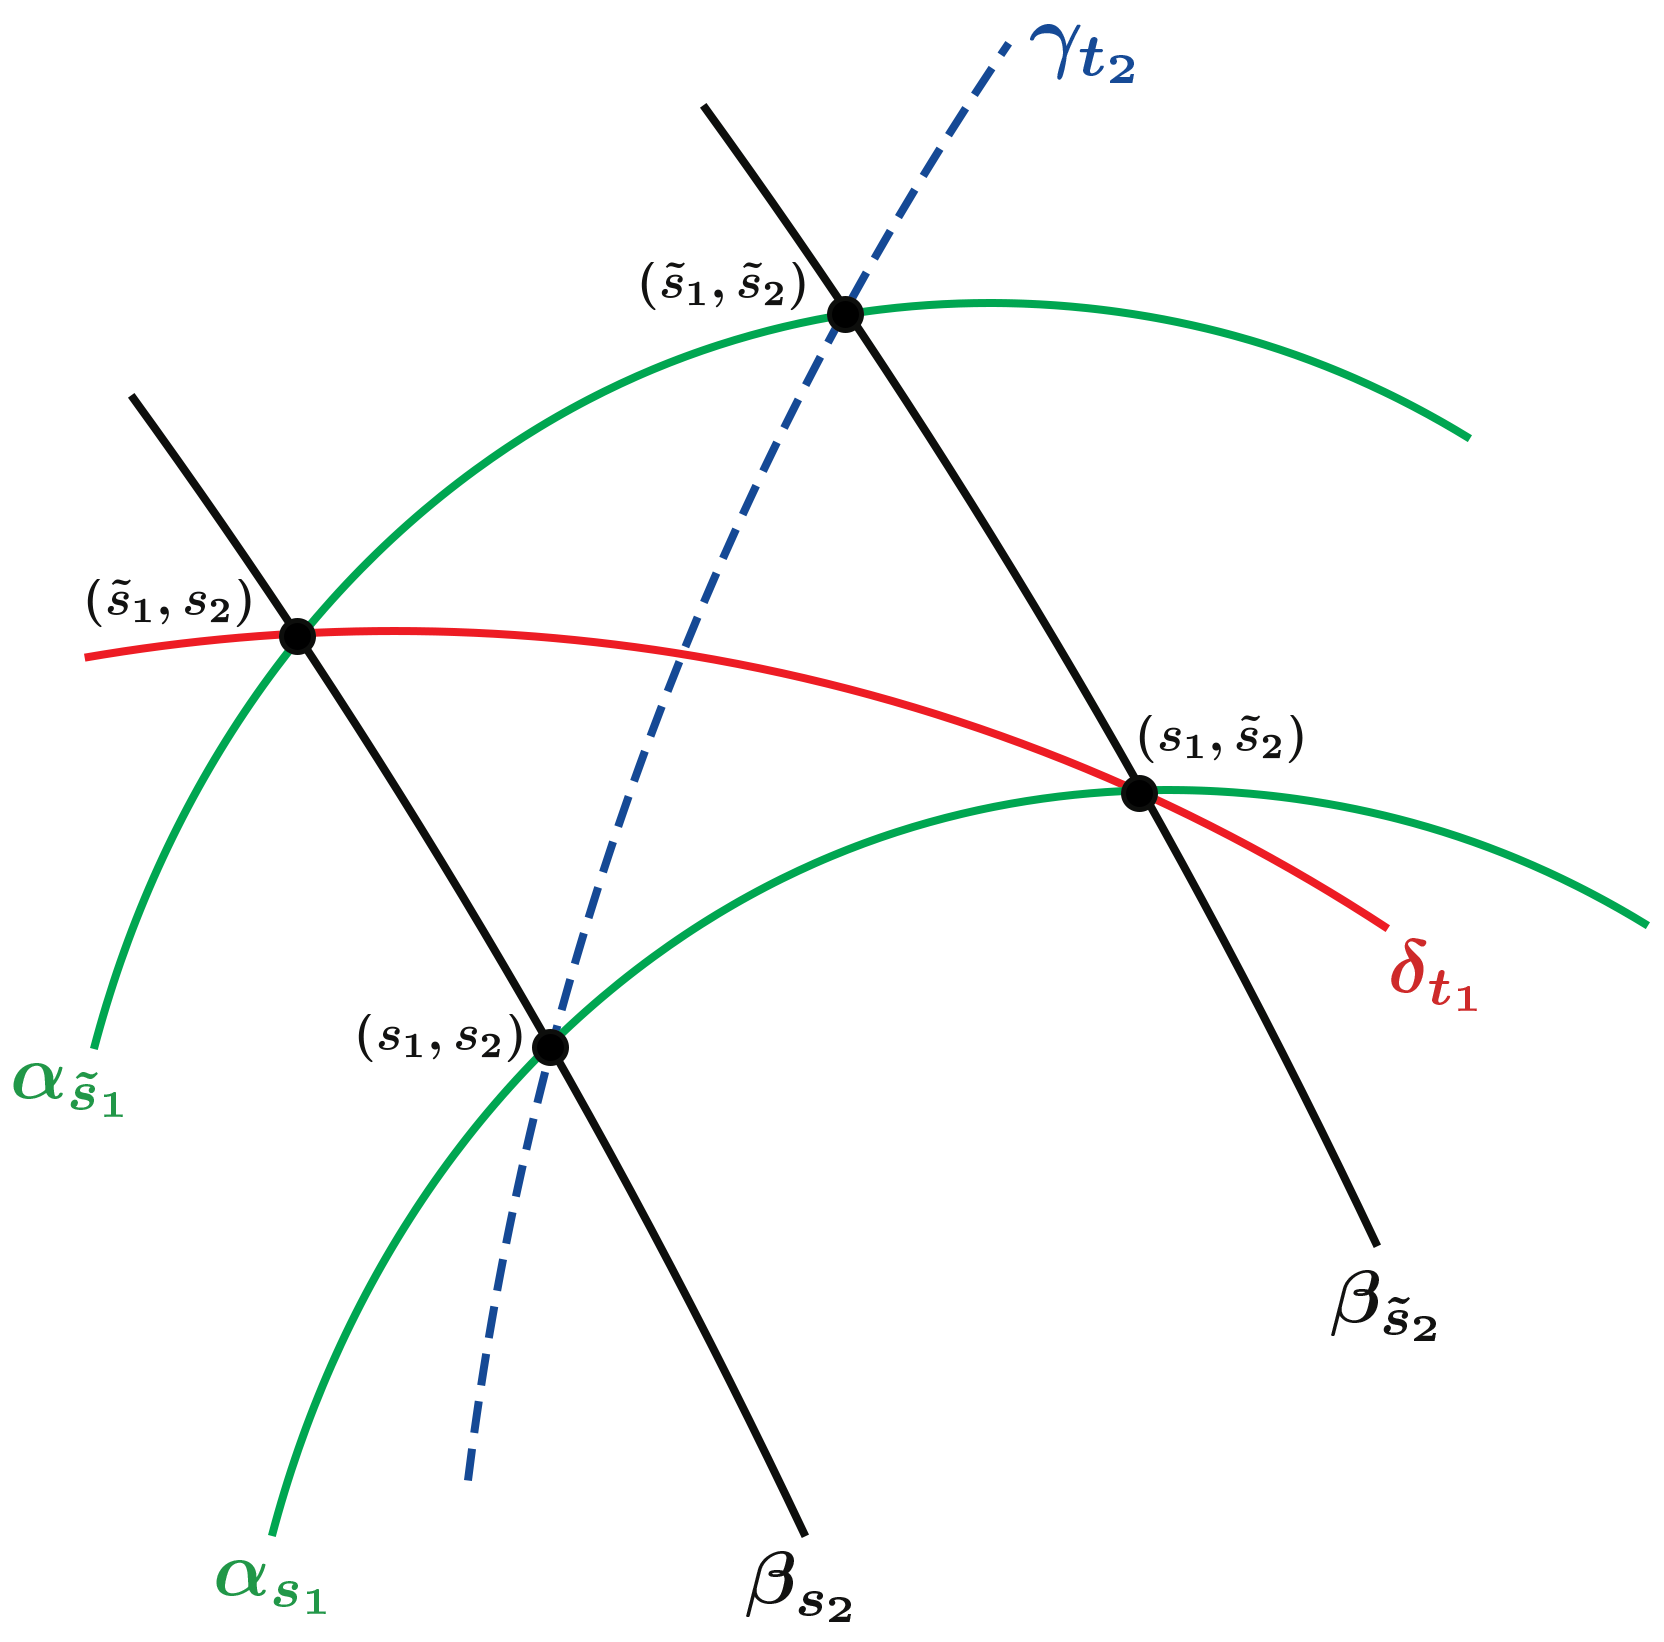
\includegraphics[width=0.5\textwidth]{diagonally_related_diagram.png}
    \caption{An illustration of the diagonal relation between two nets.}
    \label{fig:diagonally-related-diagram}
\end{figure}

\begin{theorem}[]
\label{thm:symmetric-definition-diagonal-nets}
Let $\mathcal{N}_1$ and $\mathcal{N}_2$ be two nets on a surface $\Sigma$. Then $\mathcal{N}_1$ is diagonally related to
$\mathcal{N}_2$ if and only if $\mathcal{N}_2$ is diagonally related to $\mathcal{N}_1$.
\end{theorem}

\begin{proof}
    The proof
\end{proof}

\subsection{Diagonally related parameterizations}
\pagebreak
%===========================================================
\section{Diagonally related parameterization of hyperboloids}
\subsection{Diagonally related parameterization of one-sheeted hyperboloid}
\subsection{Diagonally related parameterization of two-sheeted hyperboloid}
\pagebreak
%===========================================================
\section{Isometric deformation of circular cross sections of hyperboloids}
\section{Isometric deformation of one-sheeted hyperboloid}
\section{Isometric deformation of two-sheeted hyperboloid}
\begin{theorem}
\label{thm:affine-transformation-hyperboloid}

\end{theorem}
%===========================================================
\section{Further related work}
\subsection{Confocal paraboloids}
\section{Discrete confocal quadrics}
An interesting relation to nets on surfaces is the notion of a \textit{map} \cite{} which is an embedding of a connected
graph or multigraph $X$ into a surface $\Sigma$, such that all of the components of $\Sigma \setminus X$, called
the faces of the map, are homeomorphic to unit disks. The face-size $m$ and the vertex-degree $k$ give its type $\{m, k\}$.
\pagebreak
%===========================================================
\appendix
\section{Quadric hypersurfaces}
\label{appendix:quadrics}
\pagebreak
%===========================================================
\section{Curvature line parameterizations}
\label{appendix:curvature-lines}
\pagebreak
%===========================================================


%===========================================================
% Set page style to "tocstyle"
\pagestyle{tocstyle}
\addcontentsline{toc}{section}{References}
\bibliographystyle{alpha}
\bibliography{refs}
%===========================================================


\end{document}
